\section{\label{sec:aufbau}Setup and implementation}
Firstly, our task involves adjusting a dark-field microscope as depicted in Fig.~\ref{fig:aufbau}. 
The necessary optical instruments are already prepared for this purpose. 
Initially, adjustment is done without the dark-field mask, in bright-field mode. 
The sample can be moved in all three spatial directions using a finely adjustable sample holder. 
Additionally, the second objective from the light source is movable. 
This allows bringing the sample into focus of the first objective and then fine-tuning 
the focus by adjusting the position of the objective behind the sample. 
The camera signal from the sensor at the back of the setup is projected onto a screen. 
The detailed procedure is described in the results section and will not be further discussed here. \\
After successful adjustment, images of a test sample are captured using the camera, with recordings 
made in both bright-field and dark-field modes. 
The influence of light polarization is also examined by adding a linear polarizer behind the light source. \\
In the first part of the experiment, the dark-field microscope is adjusted, and qualitative observations are made. \\ \\
Once the camera images are reviewed and the focusing expectations are met, 
the transition to quantitative measurement can be made. 
The experimental setup is expanded, with the light hitting the camera split using a beam splitter. 
With the help of two mirrors, this sub-beam is directed onto the entrance slit of a spectrometer, 
enabling the spectroscopy of the light scattered by the nanorod ensemble. 
The sample was created using electron beam lithography and a deposition process, 
situated on a cover glass. 
The structure of the sample has a height of $35\,\si{nm}$ and is composed of silver. 
Due to the writing and deposition process, the structure is planar and consists of nanorods with 
widths $W$ of $70\,\si{nm}$ and $90\,\si{nm}$. 
The length of the nanorods varies between $70,\si{nm}$ and $140,\si{nm}$ and is denoted as variable $L$. \\
\begin{figure}[h!]
    \centering
    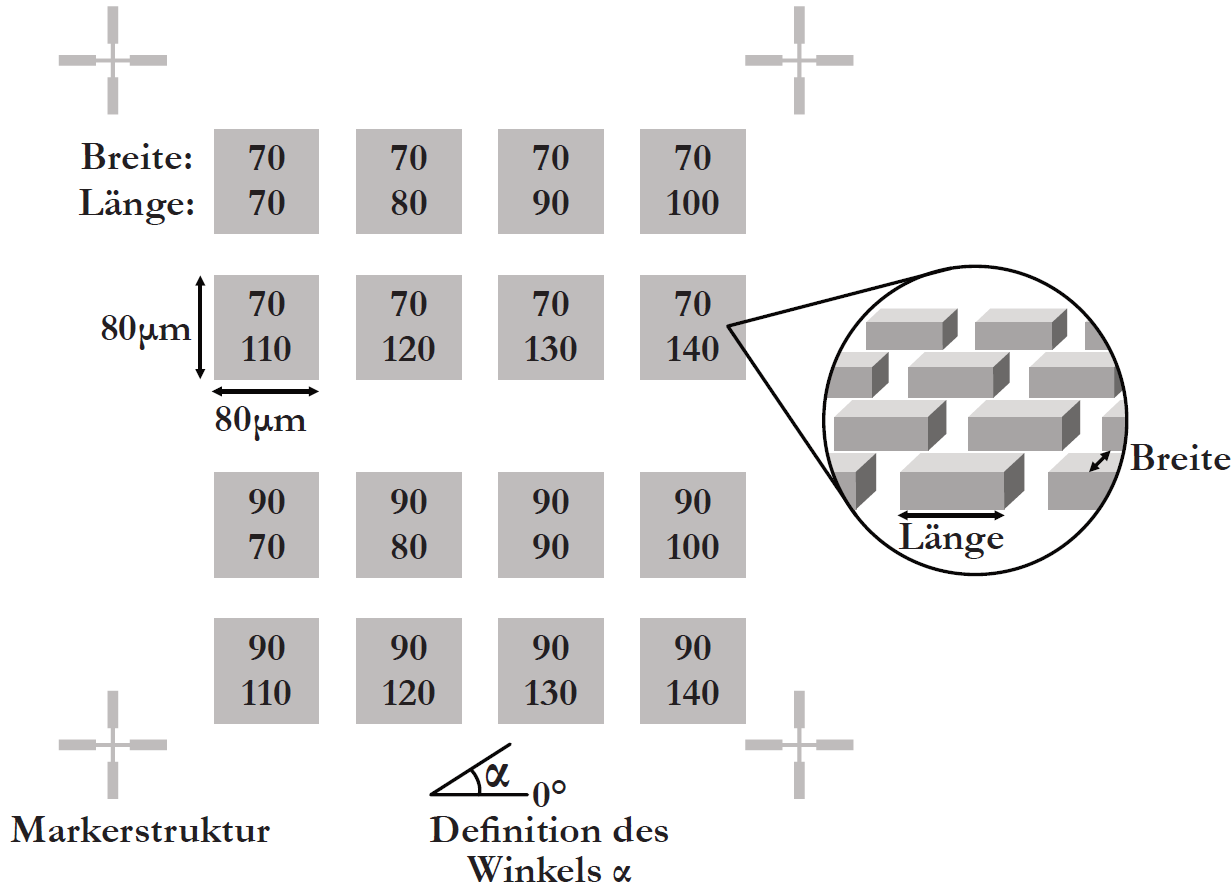
\includegraphics[width=0.6\textwidth]{Proben.png}
    \caption{\label{fig:proben}A diagram of the nanorod ensemble sample fields. 
    The first two rows feature rods with a constant width, while the length increases by $10\,\si{nm}$ per field. 
    The same applies to the lower two rows, with the width increasing to $90\,\si{nm}$.}
\end{figure} \FloatBarrier
Figure \ref{fig:proben} illustrates an overview plan of the sample, 
including the parameters of the rods in each field. 
Each field has dimensions of $80\,\si{\mu m}\times 80\,\si{\mu m}$ and contains thousands of identical nanorods. 
This arrangement allows for ensemble measurements of the scattering spectra of the rods in the respective field. \\
To ensure that only the scattering spectrum of a single sample cluster reaches the entrance slit of the spectrometer, 
a reference point is initially sought using the camera and the widely opened entrance slit. 
This reference point can be refined by closing the entrance slit. 
The positions of the mirrors and the lens in front of the spectrometer are adjusted such that a sharp sample image 
is formed in the spectrometer (verifiable in the zeroth diffraction order). 
This reference point is marked on the camera image. By shifting the sample stage, the desired scattering spectrum 
of a sample field can be directed to the spectrometer using the marker. \\
For each sample field, the scattering spectrum of the first diffraction order is recorded, with the incident 
light being unpolarized or linearly polarized at $0^{\circ}$ or $90^{\circ}$. 
The polarization angle to the sample is defined in Fig.~\ref{fig:proben}. 
Finally, the lamp spectrum is recorded in each position of the polarizer, as well as the dark spectrum without any illumination. 
All measurements are conducted without ceiling lighting. \\
Altogether, in the second part of the experiment, our adjusted dark-field microscope is 
utilized with a spectrometer to investigate the scattered light from nanorod samples 
in the first diffraction order.
The dependence of the results on the polarization of light, as well as the influence of the lamp spectrum, 
will be presented and discussed in the following chapter. \\

